\chapter{Digital Communications and Spectrum Sensing Overview}
This chapter will introduce various fundamental topics that were taken into consideration in the design of the aerial software defined radio platform developed in this MQP. The topics proposed include spectrum allocation, energy detection, wireless transmitter localization, software defined radio, and aerial flight platform.

\section{Spectrum}
Wireless communications are transmitted through the use of the electromagnetic spectrum. The spectrum consists of a multitude of frequency bands that have been allocated for specific uses.

\subsection{Spectrum Usage}
The spectrum of radio frequencies used for wireless communications is managed by the government to promote efficient use and net social benefit. The National Telecommunications and Information Administration (NTIA) and the Federal Communications Commission (FCC) regulates the allocation of these frequencies in the United States as shown in Figure \ref{fig:freq_chart} \cite{FCC_Info}. 
\begin{figure}[ht]
\centering
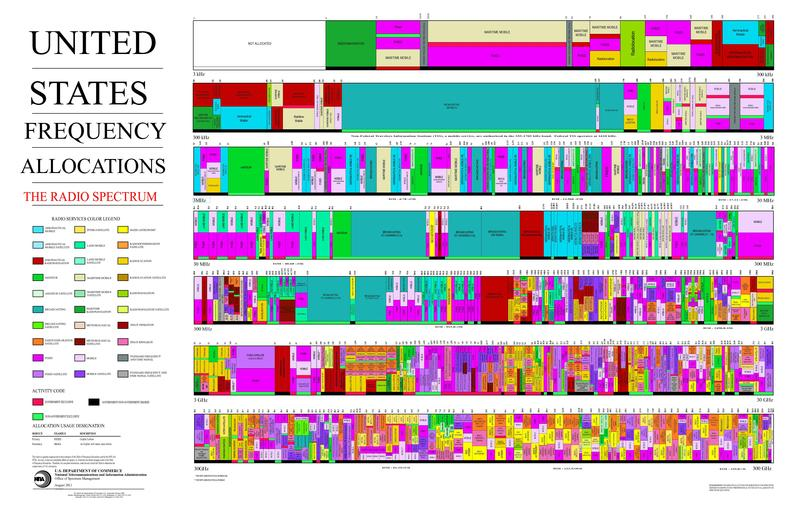
\includegraphics[width=0.70\textwidth]{img/the_radio_spectrum.jpg}
\caption{United States Frequency Allocation Chart \cite{FCC_Info}}
\label{fig:freq_chart}
\end{figure}
As seen from Figure \ref{fig:freq_chart}, the spectrum is divided into smaller chunks where only specified entities can utilize legally. The usage of each chunk is determined by whether the NTIA and FCC require a license to use the band or not. Only operators with a license from the government can operate in the licensed bands, with uses that include AM broadcasting, FM broadcasting, and cellular communication. However, unlicensed bands are open to any entity that wants to utilize them, but they must still follow certain guidelines for usage. Technologies that use unlicensed bands include microwave, bluetooth, and WiFi. \textbf{Maybe talk about the history of this a little, why it's split up like this and why the certain bands were unlicensed}

\subsection{WiFi}
WiFi first came about in 1985, when the FCC decided to open up several bands of wireless spectrum for use without a government license. In the early 1990s, the Institute of Electrical and Electronics Engineers (IEEE) realized that wireless communications needed to be standardized. A committee was formed that focused on providing a reliable, fast and robust wireless solution that would be able to scale for years to come. Therefore, the IEEE made an addition to its 802 standard which is used for local area networks, and thus the 802.11 standard was created in order to assure these things. Since then, there has been multiple iterations of the standard, and five sub-standards have been established for wireless communications called:802.11a, 802.11b, 802.11g, 802.11n, and 802.11ac. \cite{bergieee}

The first creation of the standard was 802.11 which was origionally created in 1997. The data rate was capped at 2 Mbps and transmitters transmitted on a frequency from 2.4 to 2.483 GHz. These transmitters used time-division duplexing which allows them to send uplink and downlink wireless traffic on the same RF channel. The transmitters also use interference mitigation techniques such as DSSS and FHSS which are protocols that switch wireless channels when there is other wireless interference present on that channel.

In addition to this, all the wireless standards also use a media access layer which is also known as the MAC layer.  This layer is used to assist the transmission by providing frame synchronization, and ecrypyion.  802.11 uses ecryption by using Wired Equivalent Privacy or WEP.  WEP consists of a 40 bit key that is used in order to access communication with a Wi-Fi transceiver.

WEP encryption, dynamic frequency selection, and the OFDM preamble are all have all been carried on from one standard to the next.  However, WiFi traffic can be transmitted using a variety of bandwidths dependant on their respective 802.11 standard.  Wi-Fi traffic can transmit using a 20 MHz, 40 MHz or 80 MHz bandwidth dependant on their 802.11 standard. 
\begin{table}[ht]
\centering
\caption{WiFi Protocols.  This table outlines the bandwidth, frequency spectrum and modulation type of each corresponding 802.11 interface. As the wifi protocols become newer from starting with 802.11a and ending with 802.11ac as the most recent, the protocols utilize wider bandwidths for communication, and offer a range of operating frequencies. MIMO-OFDM was also developed for later 802.11 protocols such as 802.11n and 802.11ac in order to support multipath propagation.}
\label{table:wifi_protocols}
\begin{tabular}{|l|l|l|l|}
  \hline
  Interface & Bandwidth (MHz) & Frequency Spectrum (GHz) & Modulation \\ \hline
          802.11a &              20 &                  5 &       OFDM \\
          802.11b &              20 &                2.4 &       DSSS \\
          802.11g &              20 &                2.4 &       OFDM \\
          802.11n &          20, 40 &            2.4 / 5 &  MIMO-OFDM \\
         802.11ac &      20, 40, 80 &                  5 &  MIMO-OFDM \\ \hline
\end{tabular}
\end{table}\par
These transmissions can vary when it comes to the entire frames information. However, each standard has the same preamble that signifies the start of a transmission, and what central freuency the transmission is on.  For 802.11, a wifi transmission is concentrated in one or more 20 MHz wide wifi channels or bins. At the 2.4 GHz band, Wi-Fi is allocated throughput 11 wireless channels ranging from 1 to 11.  However, only 3 of these channels (1, 6, and 11) are used due to each channel only being 5 MHz wide.  Since transmissions on the 2.4 GHz band are 20 MHz wide, the utilized channels are spaced enough to mitigate co-channel interference. This is shown in Figure \ref{fig:2.4GHz_channel}.
\begin{figure}[ht]
\centering
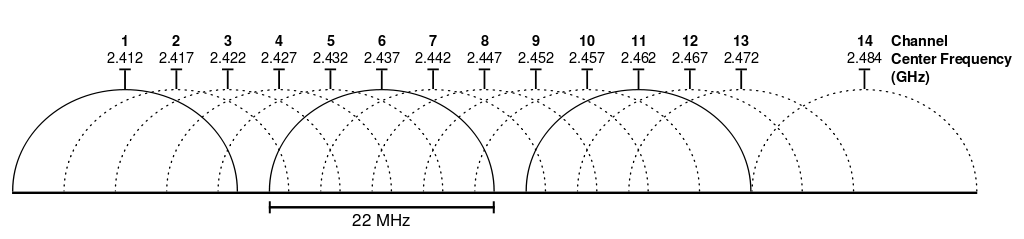
\includegraphics[width=0.70\textwidth]{img/2_GHz_Channels.png}
\caption{This image shows the allocation for 802.11 channels in the 2.4 GHz band. Each channel is 20 MHz wide and also has 10 MHz allocated as a gaurd channel. Channels 2-5 and 7-10 are not used as a wireless channel since it would be overlapping in 2 primary wifi channels.}
\label{fig:2.4GHz_channel}
\end{figure}
Also, for protocols 802.11a, 802.11n and 802.11 ac, they also use the 5 GHz frequency band which contains a range of 45 channels from 36 to 165 spanning spectrally from 5180 MHz to 5825 MHz.  This is shown in Figure \ref{fig:5GHz_channel}.
\begin{figure}[ht]
\centering
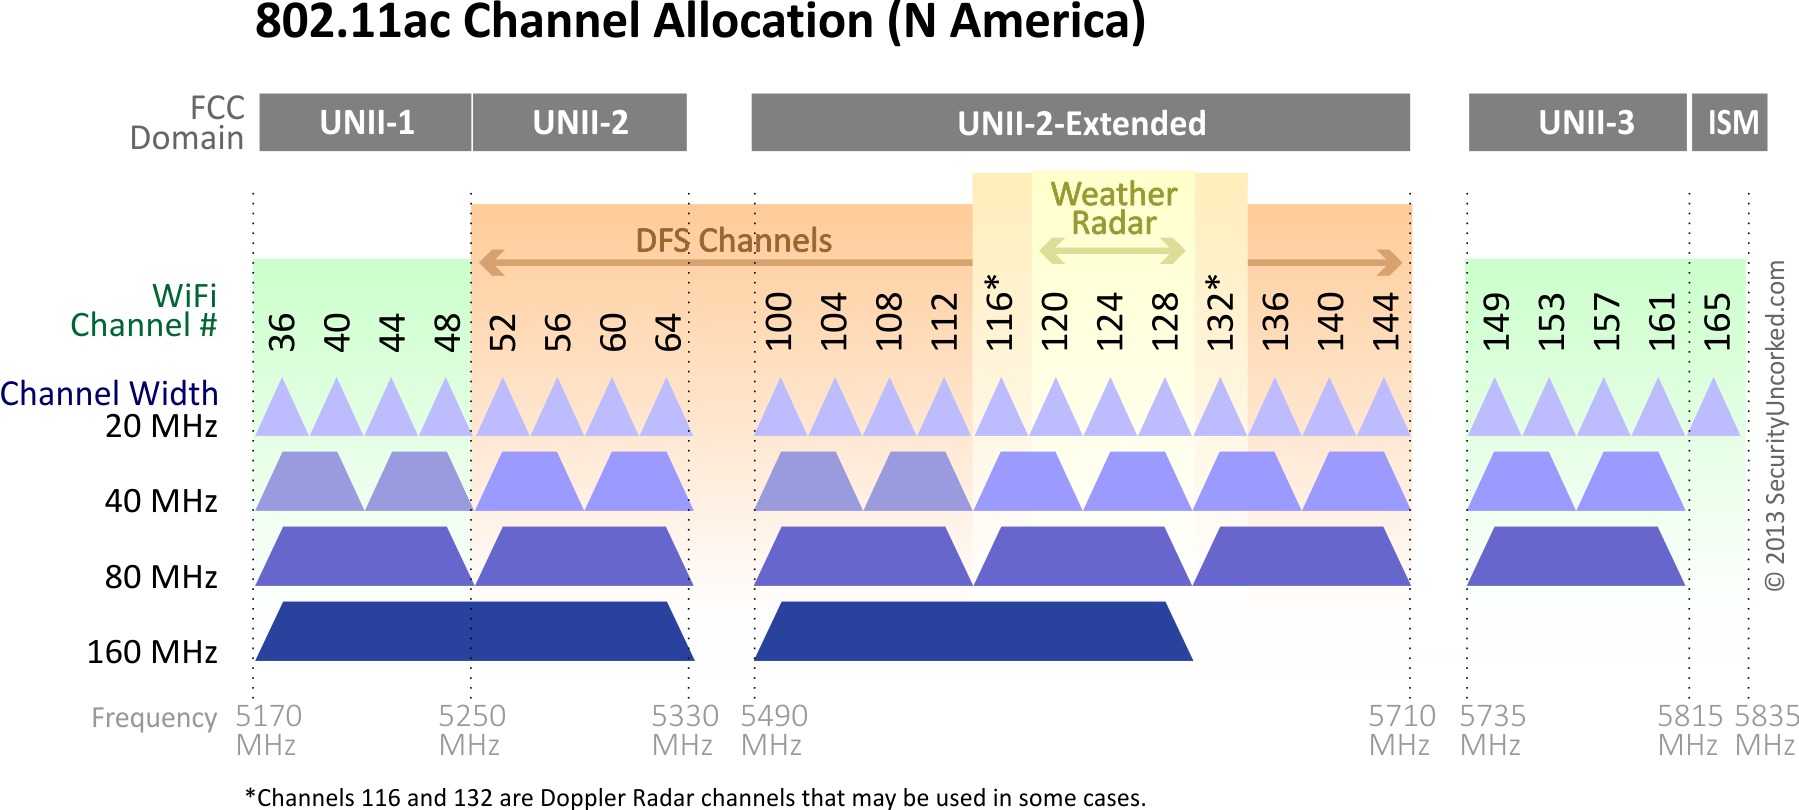
\includegraphics[width=0.70\textwidth]{img/5_GHz_Channels.png}
\caption{The 5GHz band allocates channels for higher bandwidth transmissions.  Wi-Fi channels at 5GHz cater to transmitting information at either 20, 40 or 80 MHz. Each wifi transmission on a specified channel will adapt to a higher or lower bandwidth setting based on the corresponding signal strength and interference between a transmitter and receiver.}
\label{fig:5GHz_channel}
\end{figure}
What first signifies a transmission on any of these wifi channels is the detection of the OFDM PLCP preamble which signifies which channel the information is being transmitted on. This preamble consists of  In addition to the preamble, you could also decode the information from the Data fields, however, all of that data is usually encrypted so that it prevents any unauthorized user from accessing it. \cite{wifi_book}

\subsubsection{MAVLink}
The Micro Aerial Vehicle Link (MAVLink) protocol is a free open source wireless communication protocol for controlling small unmanned aerial vehicles. This protocol first came about in 2009 by Lorenz Meier under LGPL license. \cite{MAVLINK_Website}  This protocol was designed to be a lightweight, header-only message marshaling library.  MAVLINK was first most commonly used with autopiloting software, but is trying to become the worldwide standard in drone communication. This communication protocol consists of communication with a slave drone and a master ground controller.  MAVlink controllers most commonly transmit data on the 2.4 GHz band along-side 802.11 wireless communications. Therefore, an airbourne receiver must be able to classify what type of signal it has received. To classify a MAVLink transmission, this can be done by demodulating MAVLink's GFSK modulated data, and decoding its data frame. 
\begin{figure}[ht]
\centering
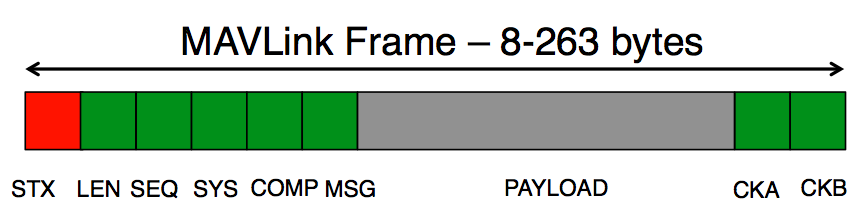
\includegraphics[width=0.70\textwidth]{img/mavlink-packet.png}
\caption{MAVLink Transmission Frame. The red STX frame signifies the start of a transmission. This frame will always be an 8 bit code of 0xFE used for start of frame detection. The following parameters give information about the payload such as it's size and who the data was meant for.  The payload category is a data field which contains a library-based command for the drone to perform.}
\label{fig:MAVlink_frame}
\end{figure} \par
\begin{table}[ht]
\centering
\begin{tabular}{|l|l|l|l|}
  \hline
  Byte Index & Content & Value &  Purpose \\ \hline
          0 &	Packet start sign &                  0xFE &       Indicates start of a new packet\\
          1 &   Payload length &                0 - 255 &       Indicates length of the following payload \\
          2 &   Packet Sequence &               0 - 255 &       Enables packet loss detection because each component counts up its send sequence \\
          3 &   System ID &            1 - 225 &  Identifies the sending system; enables multiple platforms to use the same network \\
          4 &   Component ID &         0 - 255 &  Identifies the sending component; allows for multiple components on the same platform \\
          5 &	Message ID &		   0 - 255 &  Identifies the message being sent defines the payload and how it should be decoded \\
          6 - n+6 &	Data & 			   0 - 255 & Data of the mesasge depends on message ID \\
          n+7-n+8 & Checksum & & ITU hash of bytes including MAVLINK parameter computed from message fields to prevent decoding from a different protocol version \\ \hline
\end{tabular}\end{table}
\par
Also, opposed to WiFi signals, MAVLink transmissions are all non-encrypted, making it vulnerable to things such as network attacks or an unauthorized user operating the drone. Any user can send signals to a drone using a GFSK transmitter and the drone has no knowledge on who the correct user \cite{mavlink_vuln}.

\subsection{GPS \textbf{Needs more content}}
Global Positioning System, or GPS, provides highly accurate location information to a user with a receiver module. This technology was developed during the height of the cold war in the 1960s \cite{gps_info}. GPS works by using a network of 24 satellites that are transmitting on 1575.42Mhz using a division coding scheme. The individual satellites send out information such as the current system time, and their locations. Given the locations of the satellites, as well as the calculated time of travel from the satellites to the receiver, the GPS receiver then performs localization based on this received information. The accurate time stamping required to perform this localization is only possible because each GPS satellite is capable of maintaining a highly accurate clock, and each receiver determines its current time through the interpretation of satellite data. This accurate clock information is used for the synchronization of clocks across cellular telephone systems, and other time critical applications \cite{GPS_Book}.

\section{Spectrum Sensing}
As described in the previous section, the electromagnetic radio spectrum is becoming increasingly crowded, with this issue only accelerating as the Internet of Things becomes more widespread \cite{sensing_iot}. With the conventional approach of spectrum management, users are assigned a specific frequency band. This method becomes less sustainable with the increasing number of users, especially in the unlicensed frequency bands. In order to combat this, Cognitive Radio (or CR) was created to utilize spectrum more efficiently \cite{wyglinski_book}. Cognitive radios are designed to provide a highly reliable connections for all users of the network, by sensing what frequencies are being used at any given moment, and utilizing the unused parts of the spectrum. The types of signals to be sensed are divided into two different groups: uncooperative users and cooperative users \cite{spectrum_sense_methods}. \par
The process of spectrum sensing is made more complicated by uncertainties in the received data, including channel uncertainty and noise uncertainty. With channel uncertainty, the received signal strength can fluctuate based on characteristics of the channel, such as channel fading or shadowing. Noise uncertainty refers to the fact that the power of the noise is unknown to the receiver, making it difficult to achieve a specific sensitivity \cite{spectrum_sense_methods}. In order to have a functioning CR, both uncertainties need to be addressed. \par
As the types of signals to be sensed are split into non-cooperative and cooperative systems, so too are the methods of sensing. The present MQP involves passive sensing of the spectrum, where only the methods concerning the former will be discussed.

\subsection{Energy Detection}
The simplest method of non-cooperative sensing is energy detection. In this approach, the power spectral density (or PSD) of the received signal is taken\cite{sensing_energy}. The PSD represents the measure of a signal’s intensity in the frequency domain computed through the fast fourier transform of a signal. This is then bandpass filtered to contain only the frequency bands being watched. These frequency bands are then integrated, to determine how much energy is present in the band. If this passes a certain threshold, the frequency band is marked as occupied. A MATLAB example of Energy Detection is provided in Appendix \ref{app:energy_detection}, and a flow diagram of Energy detection is shown in Figure \ref{fig:energy_detection}.
\begin{figure}[ht]
\centering
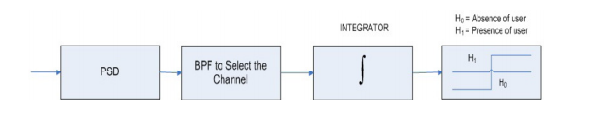
\includegraphics[width=0.70\textwidth]{img/energy_detection.png}
\caption{Flow diagram of energy detection.}
\label{fig:energy_detection}
\end{figure}\par

This method of detection is the most simple as it does not require information about the signal ignoring key aspects of signals such as modulation method and pulse shaping. Because of this, it is the simplest detection method to implement. However, an assumption made in using energy detection is that the signals being searched for have significantly more power than the noise and interference of the channel. This does not always prove to be true. In addition to this, energy detection cannot be used to distinguish signals using the frequencies measured, as no pulse shape information is determined.

\subsection{Matched Filter}
Another approach to spectrum sensing is through the use of matched filters. Matched filters are designed to maximize the signal to noise ratio (SNR) given an input signal, which will be called $s_{in}$ \cite{sensing_energy}. To sense signals through matched filtering, prior knowledge of the reference signal (or $s_{ref}$) to be detected must be known. The $s_{in}$ will then be correlated with $s_{ref}$. This produces a value m, that will be compared to a threshold value. This process is described in Equation \ref{eq:matched} below and in Figure \ref{figure:matched_filter}
. N represents the length of the reference signal, in samples. 
\begin{align} \label{eq:matched}
    m &= \sum_{k = 0}^{N}s_{in}[t-k]s_ref[N-k] 
\end{align}
\begin{figure}[ht]
\centering
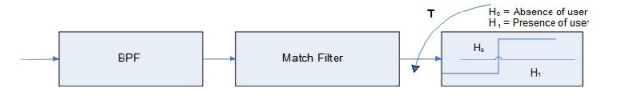
\includegraphics[width=0.70\textwidth]{img/match_filter.png}
\caption{Flow Diagram of matched filter. WORDS}
\label{figure:matched_filter}
\end{figure}\par
Matched filters rely on prior knowledge of the characteristics of signals to be detected, otherwise this method will not be accurate. The prior knowledge constraint limits the use of signal detection when unexpected signals are involved. Furthermore, matched filter detection is optimal with stationary gaussian noise to hinder distortion. This will limit the real world applications for signal detection with matched filtering as most channels are time-varying and non-gaussian \cite{channel_fade}. A MATLAB example of Energy Detection is provided in Appendix \ref{app:matched_filter}.

\subsection{Cyclostationary Feature Detection} \label{Cyclostationary Feature Detection}
Cyclostationary Feature Detection (or CFD) depends on the fact that all communication schemes have some sort of signal repetition as a core aspect. A signal with this kind of repetition is called a Cyclostationary Process\cite{cyclostat_journal}. Because of this property, when you correlate the signal with itself (or autocorrelation), there will be repeated peaks. The periodic nature of the signal also means that the autocorrelation will be periodic as well. This allows it to be expressed as a Fourier Series, called the Cyclic Autocorrelation Function (CAF) and denoted by $R_x^\alpha(\tau)$\cite{cyclostat_text}.\par 

\begin{align}\label{eq:caf}
    R_x^{\alpha(\tau)} &= lim(t->\infty) \frac{1}{T} \int_{-T/2}^{T/2} R_x(t,\tau)exp(-j2\pi\alpha t dt)
\end{align}

Where $R_x(t,\tau)$ is the autocorrelation function of x at t with x at $\tau$. This function gives us an understanding of the times when the signal repeats, but is missing vital information of the repeated frequencies. By taking the fourier transform of $R_x^\alpha(\tau)$, one can get a better understanding of the frequencies in the Cyclostationary Process. This is denoted as $S_x^\alpha(f)$, and is equal to \cite{cyclostat_text}:  \par

\begin{align}\label{eq:scf}
S_x^\alpha(f)=\int_{-\infty}^{\infty} R_x^\alpha(\tau)exp(-j2\pi f\tau d\tau) 
\end{align}
\par

This is called the Spectral Correlation Function (SCF). When it is normalized, it becomes the Spectral Coherence Function (SOF) \cite{cyclostat_text}:
\begin{align}\label{eq:caf}
C_x^\alpha(f) = \frac{ S_x^\alpha(f)}{ (S_x^\alpha(f+\alpha/2) S_x^\alpha(f-\alpha/2))^{1/2}}
\end{align}\par
The SOF is from between 0 and 1, and represents the strength of the periodicity at that point. By plotting this value, the unique response of the Cyclostationary Process can be found, allowing for it to be categorized.\par

One of the major benefits of CFD is that it is not nearly as affected by noise. Under the generally held assumption that noise is white and Gaussian, there is no periodic response, and as such noise is not factored into CFD. Example plots from an implementation of CFD are shown below. \par
\begin{figure}[ht!]
\centering
  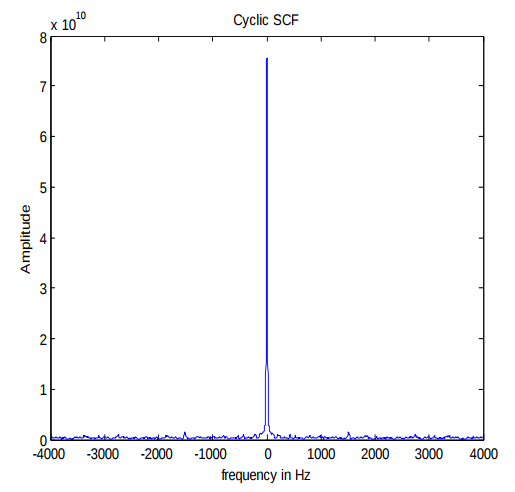
\includegraphics[scale=0.4]{img/cyclic_scf.png}
\caption{The SCF of a simple signal}
\label{fig:cyclic_scf}

\end{figure}
\begin{figure}[ht!]
\begin{minipage}{.5\textwidth}
  \centering
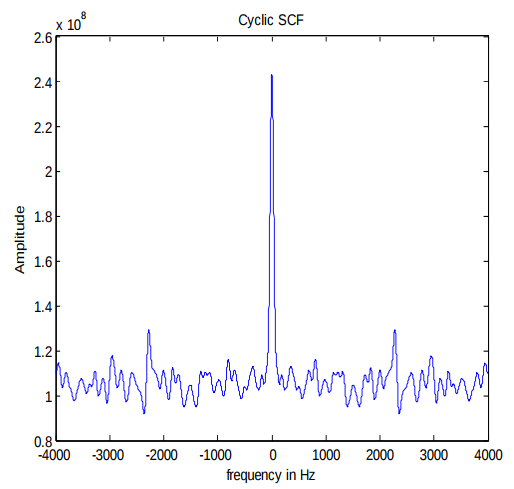
\includegraphics[scale=0.4]{img/cyclic_scf_bpsk.png}
\caption{The SCF of a simple signal, modulated with BPSK.}
\label{fig:cyclic_scf_bpsk}
\end{minipage}
\begin{minipage}{0.5\textwidth}
\centering
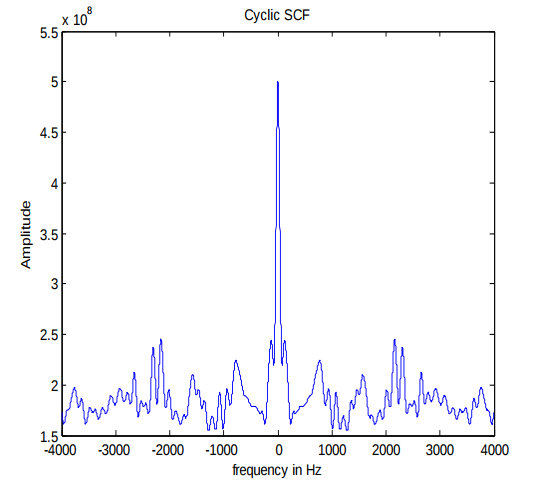
\includegraphics[scale=0.4]{img/cyclic_scf_qpsk.png}
\caption{The SCF of a simple signal, modulated with QPSK.}
\label{fig:cyclic_scf_qpsk}
\end{minipage}
\end{figure}

% \begin{figure}[ht!]
% 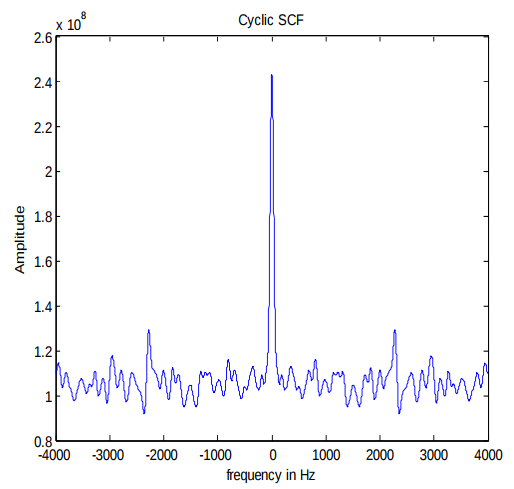
\includegraphics[scale=0.4]{img/cyclic_scf_bpsk.png}
% \caption{cyclic scf BPSK \textbf{Needs to be 2-3 sentences -Narut}}
% \label{fig:cyclic_scf_bpsk}
% \end{figure}

% % \begin{subfigure}{0.5\textwidth}

% %\end{subfloat}
% \end{figure}
% % \begin{figure}[ht]
% \centering

% \end{figure}
% \begin{figure}[ht]

% \end{figure}

The primary downside to Cyclostationary Feature Detection is the complexity and time required to properly utilize it. The complexity lies in the number of integrals and correlations that need to be computed in order to implement CFD. In addition, the system needs to listen for signal long enough for the Cyclostationary Process to repeat. Because of these downsides, it is not common to be used on embedded systems. \par


\section{Radio Localization}
Once a signal has been identified on a measured frequency, the next step is localization. Localization refers to the act of determining the location of a transmitted signal \cite{local_conf}. There are many different methods for localization. However, many of them become impractical for mobile passive sensing. In the following section, a variety of localization techniques will be discussed, as well as the practicality of implementing each of them.\par
For each of the techniques discussed below, the same basic concept is used. Three different receivers are placed around the transmitter being located, as shown in Figure \ref{fig:node_localization}.  They will be called stationary nodes and the unknown node, respectively. Each stationary node gets information about its location relative to the unknown node simultaneously. For Time Difference of Arrival (TDoA), Time of Arrival (ToA), and Received Signal Strength (RSS) Localization, each stationary node calculates the distance to the unknown node. This information is used with the known locations of the stationary nodes to localize the unknown node. Angle of Arrival (AoA) functions differently and will be described in a separate section. \par

%12/5/16 A Page break should go here, assuming nothing changes. Max
\begin{figure}[ht]
\centering
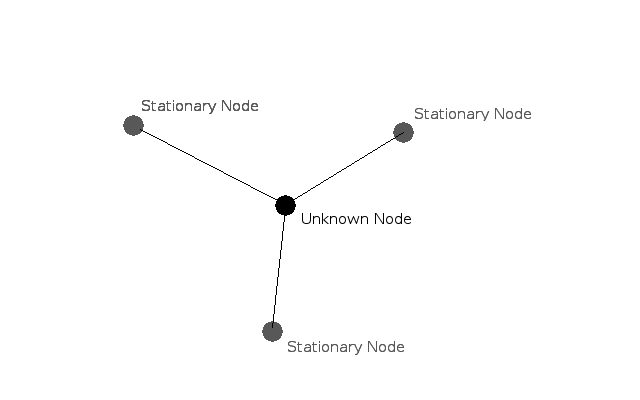
\includegraphics[scale=0.5]{img/node-localization-lines.png}
\caption{Node Localization \textbf{Needs 2-3 sentences}}
\label{fig:node_localization}
\end{figure}\par

Table \ref{table:local_methods} shows the most important details of the localization techniques that will be described. \par
\begin{table}[ht]
\centering
\caption{Localization Methods}
\label{table:local_methods}
\begin{tabular}{|l|l|l|l|}
    \hline
  Localization Method   & Mathematical Technique    & Needs Unknown Node Participation? & \\ \hline
         TDoA           & Distance                  & Yes                               & \\
          ToA           & Distance                  & Yes                               & \\
          RSS           & Distance                  & No                                & \\
          AoA           & Angle                     & No                                & \\
    \hline
\end{tabular}
\end{table}\par

%%%%%%%%%%%%%%%%%%%%%%%%%%%%%%%%% got here -Narut
In the distance-based localization techniques, each stationary node knows the unknown node is a certain distance away \cite{local_conf}, allowing for it to be anywhere along a circle, with the stationary node in the center. By finding out where all three circles intersect, the unknown node can be located. The distance of the unknown node from any of the stationary nodes is calculated using Equation \ref{eq:dist_coord}.\par 
\begin{align}\label{eq:dist_coord}
D_i &=\sqrt{(X - x_i)^2 + (Y-y_i)^2}
\end{align}\par
By plugging in the locations and calculated distance for each stationary node, a system of equations is created, making it possible to solve for the location of the unknown node.\par
%TDoA
One method of localization is Timed Difference of Arrival (TDoA) \cite{local_conf}. In this method, the unknown node transmits a signal over radio frequencies. Using the difference in the timestamp and actual time of receiving the signal, the stationary nodes can calculate the distance between each stationary node and the unknown node, using Equation \ref{eq:dist_light}. c represents the speed of light.
\begin{align}\label{eq:dist_light} 
    d &= c*(t_{actual} - t_{expected}) 
\end{align} \par
This method of localization is dependent on three things: the synchronization of the nodes involved, the participation of the unknown node, and the existence of three or more stationary nodes. In the use case presented by this MQP, the most difficult part about this implementation is the participation of the unknown node. Since the aerial platform has no communication with the object being localized, this method is impractical. \par

%%Time of Arrival
Using the Time of Arrival (or ToA) approach is similar to TDoA in concept \cite{local_conf}. Each of the stationary nodes sends a signal at a specific time, known to the unknown node, $t_0$. Using the difference in $t_0$ and the time that the base receives the signal, or $t_1$, the unknown node calculates the time the signal was in the air, and uses the speed of an electromagnetic wave to determine the distance to the stationary node, as described above. With three of these calculations, the location of the unknown node can be triangulated.\par

Like TDoA, ToA requires the synchronization of the nodes involved \cite{local_conf}. In most implementations, this is done using digital timestamps. It also requires the participation of the unknown node. Similarly to TDoA, these requirements make ToA an impractical fit for this MQP. \par

%RSSi Localization
Unlike the previous two methods, which depend on knowing the time a signal was sent, received signal strength localization uses the strength of a received signal to localize the unknown node \cite{local_conf}. Each of the stationary nodes receives the signal being output by the unknown node. Using the Equation \ref{eq:rssi} and Equation\ref{eq:rssi_dist}, the stationary nodes can calculate the distance to the unknown node \cite{rss_calc}. From this, they can triangulate the location as described before.\par
\begin{align}
\label{eq:rssi} RSSI &= 10\alpha log(d) \\ 
\label{eq:rssi_dist} d &= 10^{(RSSI-RSSI_{calibration})(-10\alpha)} + d_{calibration}
\end{align}
\par
Because RSSI localization depends on the measurement of the signal strength, it is adversely affected by sources of noise and interference, like channel fading and multipath interference \cite{local_conf}. This makes the technique have lower accuracy. The effects of noise and shifting channels can be somewhat mitigated by averaging the RSS data.

%Angle of Arrival.
\textbf{MATLAB EXAMPLE OF AoA probably needed}
Unlike the previously described methods, some localization techniques use the angle that the signal arrives at relative to a reference direction, or the Angle of Arrival (AoA) \cite{local_aoa}. To use this method, antenna arrays or directional antennas are used to determine the angle at which the signal arrived at. Similarly to TDoA, the stationary nodes wait for a signal from the unknown node. Using the directional antenna or the antenna array, the AoA is calculated at each stationary node. From each of these nodes, a ray can be drawn originating from the node that follows the angle of arrival. The unknown node is located based on where the rays intersect.

\begin{figure}[ht]
\centering
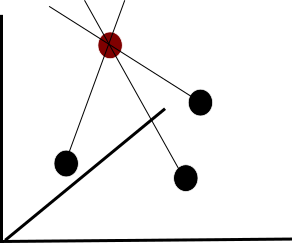
\includegraphics[scale=0.5]{img/path4188.png}
\caption{Angle of Arrival Diagram}
\label{fig:aoa_diagram}
\end{figure}\par
AoA localization consists of similar issues as other techniques. Noise and channel issues still come into effect. Additional issues occur if these unknowns can’t be dealt with. Another constraint is the requirement for highly directional sensing, which complicates the sensing of a signal before localizing it. This can either be done with many antennas or a very directional antenna, but it adds complexity.

\section{Kalman Filtering}
In the previous section, the localization techniques discussed were discussed mainly on the merits of the technique itself, assuming that the numbers used in the techniques are as good as they can be. Usually, this isn't the case \cite{kf_book}. Changing environment conditions and noisy sensors introduce errors that are hard to predict, and thus hard to mitigate. This is one of the motivations of Kalman filters, as well as the field of error estimation in general. In addition, Kalman Filters are frequently used as a way to control a system, using the estimate as feedback. Any applications relevant to this project are solely estimation-based, so the rest of this section will focus on this aspect of Kalman filters. \par

In most situations, the known information of a system is a combination of sensor values and a model of what the sensor values should be. The sensor values are imperfect, and have some amount of noise \cite{kf_pictures}. The model, based on some fundamental assumptions, is too imprecise to perfectly apply to the situation. By choosing some middle value in between the measurement and the prediction, a more accurate value can be produced. The Kalman filter is one way to decide which middle value to use \cite{kf_robots}. It applies only to linear systems. Non-linear systems can be linearized and used as an input to a Kalman filter, in which case it is called an Extended Kalman filter. The math for Extended Kalman filters is fairly complicated, so the focus of this section will be standard Kalman filters.\par
The equations used in a Kalman filter are shown below:
\subsubsection*{Predict:}
\begin{align}
    \vec{x} &= \matr{F}\vec{x} + \matr{H}\vec{u} \\
    \matr{P} &= \matr{F}\matr{P}\matr{F^T} + \matr{Q} 
\end{align}
\subsubsection*{Update:}
\begin{align}
    \vec{y} &= \vec{M} - \matr{H}\vec{x} \\
    \matr{S}&= \matr{HPH^T+RS} \\
    \matr{K} &= \matr{PH^TS^{-1}K} \\
    \vec{x} &= \vec{x} + \matr{K}\vec{y} \\
    \matr{P} &= \matr{(I-KH)P}
\end{align} \par

The first set of equations predicts the current state given the last state. The first equation updates the state based on the current state and current input. The vector $\vec{x}$ is the state of the Kalman filter. This has the values being filtered. $\vec{u}$ is the value of the controls being used to alter the state. In our application, this is 0. $\matr{F}$ is the state transition matrix, which determines how the different states interact with each other.  $\matr{H}$ is the control matrix. The second equation updates the covariance matrix of the state, which is $\matr{P}$. $\matr{Q}$ is the covariance of the noise of the environment. \par

The second set of equations updates the Kalman filter to take into account the most recent measurement. $\vec{y}$,sometimes called innovation, is the difference between the measurement received and the last state prediction. 
$\matr{S}$ is an intermediate matrix, used so that the calculation of the Kalman gain $\matr{K}$ is not too complicated in one step. Some documentation on Kalman filtering skip this step.  $\matr{R}$ is the covariance of the noise of the model. The calculated Kalman gains are then used to update the state and state covariance to take into account the updated model and input. \par

\section{Software Defined Radio}
Due to the rapidly increasing number of users dependent on efficient spectrum allocation for communication, the use of reprogrammable radios has become an integral part of designing communication systems. Radios exist in a wide range of devices, such as cell phones, cars, televisions, garage door openers, and computers. A radio is any device that transmits or receives wireless signals that are within the radio frequency band of the electromagnetic spectrum. A software defined radio (SDR) is defined as a “radio in which some or all of the physical layer functions are software defined” \cite{sdr_forum}. Traditional hardware based radios are nearly impossible to modify post-production, and have limited ways to be repurposed. SDRs, on the other hand, are comparatively inexpensive, highly reusable, and are easily configurable to support multiple waveform standards.\par
There are multiple different families of SDRs, two of which are RTL and Universal Software Radio Peripheral (USRP). An RTL is a low cost SDR that uses a DVB-T TV tuner dongle based on the RTL2832U chip set \cite{rtl_sdr}. The DVB-T TV tuner was converted to be used as a wideband SDR using a new software driver. The RTL-SDR can be used for many applications including listening to aircraft traffic control, decoding ham radio packets, and sniffing GSM signals. The USRP is a flexible transceiver that is able to use a standard PC to prototype wireless systems. USRPs are able to prototype a wide range of single-channel and multi-input multi output (MIMO) wireless communication systems \cite{USRP_NI}. USRPs can be programmed using software frameworks including GNU Radio, Matlab, Simulink, LabVIEW, C++.\par
SDRs can be implemented on field programmable gate arrays (FPGA), digital signal processors (DSP), programmed System on Chips (SoC), general purpose processors (GPP), personal computers (PC), or other reprogrammable application specific integrated circuits (ASICs). The use of these reprogrammable technologies allows for the possibility of constant updates or dynamic radio systems without the need to add additional hardware. The primary goal of designing an SDR is to implement as much of the radio in the digital space, minimizing the use of analog components. The digital portion of an SDR performs the data compression, encoding, modulation, demodulation, decoding, and decompression in software. The only analog components are a digital to analog converter (DAC), an analog to digital converter (ADC), and a RF circuit. The RF circuitry on the transmitter consists of a smoothing filter to reduce the hard edges of the baseband signal that the DAC outputs as well as circuitry to upconvert the baseband signal. The RF circuitry on the receiver side consists of a downconverter to move the signal to the baseband as well as filters to remove noise from the signal. The DAC and ADC serve as the bridge between the analog and digital realms enabling the software defined signal to be converted to an analog one to transmit and receive, then converted back to digital on the receiving end shown below in Figure \ref{fig:sdr_flow_diagram}.
\begin{figure}[ht]
\centering
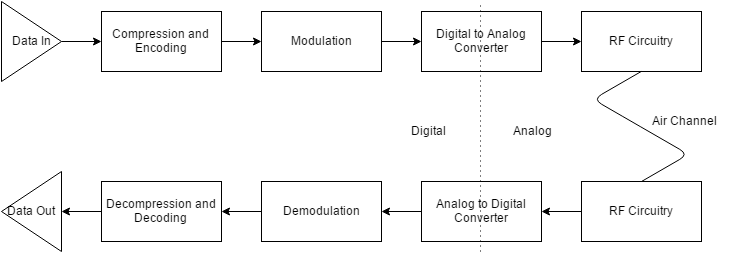
\includegraphics[width=0.70\textwidth]{img/sdr_diagram.png}
\caption{Flow diagram of an SDR with the distinction between the digital and analog components}
\label{fig:sdr_flow_diagram}
\end{figure}\par
A typical transmitter will pass a modulated signal to the DAC which will take the digital input and output a baseband analog signal. The analog signal will be upconverted to the carrier frequency in a single step or multiple steps. The receiver will take the received analog signal and downconvert it. It then passes the baseband analog signal to the ADC to convert the signal back into digital for the SDR to process. The capabilities of the ADC and DAC, such as the as the bandwidth and noise tolerance of these two components, will dictate the complexity the RF circuitry that is needed to satisfy these requirements.\par
A software defined radio, such as an adaptive radio, has the capability to be much more sophisticated than an analog counterpart. Adaptive radios are able to monitor their own performance and adjust their parameters to ensure the highest quality of service \cite{cog_radios}. A more advanced type of adaptive radio is the cognitive radio, mentioned in \ref{Cyclostationary Feature Detection}, which is able to monitor, sense, and detect conditions of their operating environment and adjust its characteristics to match those conditions. This allows the radio to provide improved performance and quality of service. These radios are able to find and transmit on open gaps in a radio spectrum. This allows for minimal interference from other sources. Cognitive radios use the trends of the channel to determine whether to switch channels or continue using the current channel. The most advanced type of adaptive radio is the intelligent radio. These radios are capable of machine learning which enables the radio to improve its algorithm for adjusting the radio's parameters based on previous experience when changes to performance or the environment occur \cite{int_radio}. The relationship between these types of radios is shown below in Figure \ref{fig:sdr_relationship_diagram}.\par
\begin{figure}[ht]
\centering
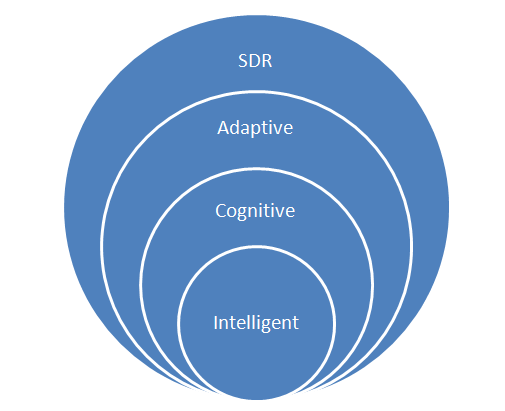
\includegraphics[width=0.70\textwidth]{img/sdr_diagram2.png}
\caption{The relationship between SDR, adaptive radio, cognitive radio, and intelligent radio}
\label{fig:sdr_relationship_diagram}
\end{figure}\par
There are three major groups of algorithms that intelligent radios are based on: machine learning, genetic algorithms, and fuzzy control \cite{amraoui2012intelligent}. Neural networks are a type of machine learning that use large group of nodes to solve problems similarly to how the human brain operates. When new information is aquired, this information is incorperated into the algoithim to be used to improve the output \cite{amini2011universal}. This technique is used to estimate the performances of WiFi networks and respond to changes in the network. Fuzzy logis is usually combined with neural netowrks that adapt to the envirnment during the operation of an intelligent radio. A fuzzy logic control system is used to find the solution to a problem given imperfect information \cite{amraoui2012intelligent}. There are three main components in a fuzzy logic controller: fuzzifier, fuzzy logic processor, and defuzzifier.The fuzzifier maps the inputs into fuzzy sets, the fuzzy logic processor determines a fuzzy output based on a set of rules, and the defuzzifier transforms the fuzzy output into a crisp output. One of the main advantages to fuzzy logic is its low complecity, which is extremely useful in real-time radio applications. Another example of an algorithm used in intelligent SDRs is the wireless system genetic algorithm (WSGA). This algorithm is a multi-objective genetic algorithm (MOGA) designed for the control of a radio by modeling the physical radio system as a biological organism and optimizing its performance through genetic and evolutanry processes \cite{rondeau2004cognitive}. Each aspect of the radio such as payload size, coding, encryption, and spreading can be considered gene that can be modified through these processes. These genes are combined into a chromosome that is used to evolve the system. The algorithm analyzes the effectiveness of the chomosome through weighted fitness functions defined by performance evaluations of the current radio channel \cite{rondeau2004cognitive}.\par
SDRs are used in a variety of different applications and are becoming more sophisticated. They are more modular than the analog equivalent and arecapable of adapting to their environment. They are also very easily updated and modified as opposed to using an analog circuit. The SDR is widely used because of these benefits over the analog design.

\section{Aerial Platforms}
The inspiration behind this MQP was to discover how much information could be gathered from the wireless spectrum when observed from the air. Aerial platforms have been used in the past for surveying tasks like geographical mapping. \cite{geomap_patent} These systems generally use a camera to capture visual images from above. To facilitate flying our sensory system, three main mobile methods of elevating the sensory unit were considered: kites, fixed-wing aircraft, and multicopters, each of which will be described in detail below.

\subsection{Kites}
A kite is a passive structure tethered to the ground that stays airborne by catching wind \cite{kite_book}. There are many different styles of kite, including parafoil, rokkaku, delta, and sled, but they all rely on the same principle to fly \cite{kite_book} \cite{kite_iqp}. Kites have near unlimited flight time and high payload capacity when operated in favorable conditions, but in exchange they sacrifice control, reliability, and maneuverability.\par
Since kites are powered by the natural wind in the atmosphere, they do not require any power to stay aloft. However, depending on the style of kite, they do require specific conditions to fly. Almost all kites need at least 2-3 mph of wind to get up into the air, and delta and rokkaku are limited to a maximum of 12-16 mph \cite{kite_iqp}. Parafoils can fly in wind up to 20 mph, but can be unstable.\par
The only control a user has over a kite in flight is changing its height by letting out or reeling in more of the tether cord. Different styles of kite have different flying angles, which impacts the amount of weight they can carry. Some kites, such as the rokkaku and delta (example in Figure \ref{fig:delta_kite}) styles, can be modified during assembly to change their angle of flight, where higher angles produce more lift. While parafoils can inherently carry more weight, they also have a low flying angle, which can be problematic in some scenarios. The preparation for flight involves assembling the kite, normally by inserting cross-bars, and unreeling the tether in an open space that allows the kite to take off.\par
\begin{figure}[ht]
\centering
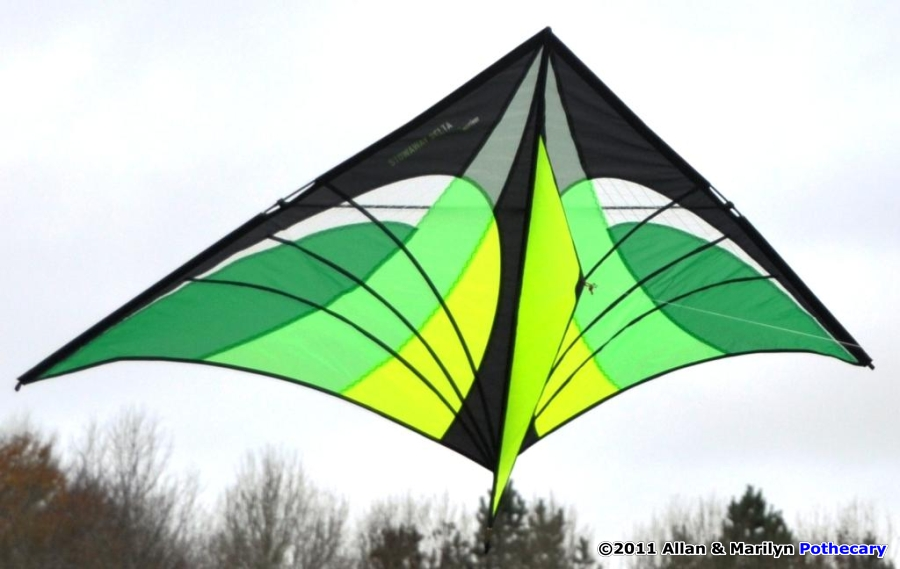
\includegraphics[width=0.70\textwidth]{img/delta-kite.jpg}
\caption{A delta style kite. Delta style kites can be configured to fly at high angles, allowing them to be flown in laterally constrained locations.}
\label{fig:delta_kite}
\end{figure}\par
Kites are, by necessity, constructed of very light materials and cannot support much extra weight in light wind situations. Again, the style of kite affects the carrying capacity: deltas can carry a moderate amount of weight, but need higher winds to stay aloft. Parafoil and rokkaku kites can carry more weight, with 10 lbs being on the low end.\par
One application of kites that concerns the carrying capacity is kite aerial photography, which consists of a camera mounted to a kite as a low-cost way to take aerial pictures. Varying flying conditions force photographers to mount cameras to many different types of kites with differing angles of flight, payload capacity, and stability. Advanced photographers also utilize mounting rigs to stabilize and sometimes rotate the cameras in flight \cite{kite_iqp}.\par
The pros and cons of a kite as a platform for the SDR system are enumerated in Table \ref{table:kite_pc}.
\begin{table}[ht]
\centering
\caption{Kite Pros and Cons}
\label{table:kite_pc}
\begin{tabular}{l|l}
  Pros & Cons \\ \hline
  cost & maneuverability \\
  flight time & deployment time \\
  payload capacity & \\
\end{tabular}
\end{table}\par

\subsection{Fixed-wing Aircraft}
A fixed-wing aircraft is a rigid structure with one or more rotors oriented forward that gains lift from the flow of air over its wings \cite{airplane_book}. A diagram showing this lift mechanism can be found in Figure \ref{fig:airfoil_lift}. This section will focus on radio controlled (RC) aircraft since they are the type being considered for use in this MQP. An RC aircraft’s movement is typically controlled by servos onboard that move flaps to change the surface of the aircraft, in turn changing the dynamics of flight and causing the plane to respond. RC aircraft are very efficient in terms of flight time to power used because the lift comes from the shape of the wings, not the speed of the motor \cite{airplane_site}. Since the lift comes from the wings, fixed-wing aircraft have a moderate flying time and can carry a moderate amount of weight, but the plane’s motion is very linear so its maneuverability is limited.\par
\begin{figure}[ht]
\centering
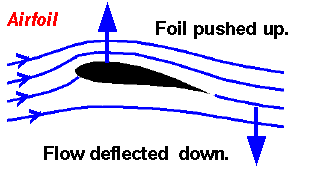
\includegraphics[width=0.70\textwidth]{img/airfoil_lift.png}
\caption{Airfoil lift generation. As air flows past the airfoil, it is forced downward, in return forcing the aircraft upward.}
\label{fig:airfoil_lift}
\end{figure}\par
The flight time of most battery powered RC fixed-wing aircraft is around half an hour assuming some aerobatics \cite{airplane_book}. In a surveying role, with the plane flying low circles, the flight time would likely increase slightly. There are also gasoline powered aircraft with small engines onboard to power the main propeller. Gasoline has a very high energy density, so it’s possible to fly for multiple hours with a gasoline powered aircraft.\par
Fixed-wing aircraft have a fairly lenient payload capacity. One thing to consider about adding payloads to fixed-wing aircraft is that since the aircraft’s flight is so heavily impacted by the body shape, any payload will need to be incorporated into the body of the aircraft to minimize airflow disturbance. To get more lift, and thus carry more weight, the plane simply needs to fly faster to force more air over the wings. This has drawbacks however, as spinning the propeller faster will drain the power source faster and decrease maneuverability.\par
Fixed-wing RC aircraft have been used in the past for similar tasks. In one example, a group of students at WPI developed a search and rescue platform using a fixed-wing RC aircraft \cite{airplane_iqp}. An example of a fixed-wing RC aircraft is shown in Figure \ref{fig:fixed_wing}.
\begin{figure}[ht]
\centering
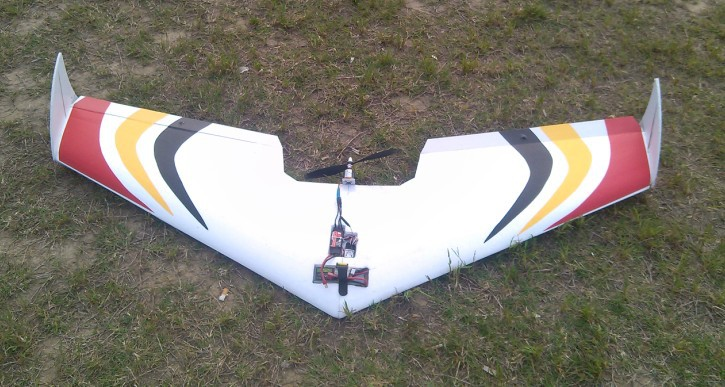
\includegraphics[width=0.70\textwidth]{img/fixed-wing.jpg}
\caption{A fixed-wing RC aircraft. This is a flying wing style craft with a rear propellor. Its flight would be greatly hindered by any protrution of a mounted system.}
\label{fig:fixed_wing}
\end{figure}\par
A fixed-wing aircraft is able to cover large distances flying laterally, but it is not able to stop mid-flight and hover in place \cite{airplane_book}. Its turning radius is often quite large, and it must not drop below a certain speed to remain airborne. While fixed-wing aircraft are mobile, they are not very agile. Most fixed-wing aircraft require a long flat runway to takeoff and land on, limiting the number of locations in which they could reasonably launch. In addition, fixed-wing aircraft are much larger and are commonly disassembled for transport.\par
The pros and cons of a fixed-wing aircraft as a platform for the SDR system are enumerated in Table \ref{table:wing_pc}.
\begin{table}[ht]
\centering
\caption{Fixed-Wing Aircraft Pros and Cons}
\label{table:wing_pc}
\begin{tabular}{l|l}
  Pros & Cons \\ \hline
  flight time & maneuverability \\
  payload capacity & cost \\
   & deployment time \\
\end{tabular}
\end{table}\par

\subsection{Multicopters}
A multicopter, sometimes also called a drone, is a flying device with two or more upward oriented rotors. A typical multicopter structure will have an even number of fixed-pitch propellers (often 4, 6, or 8), powered by electric motors placed equidistant from the center of mass \cite{multicopter_background}. To have full control over the movement of the quadcopter, at least 3 rotors are needed \cite{multicopter_dynamics_2}. The least mechanically complex of the three devices investigated here, multicopters rely solely on software control of the rotors for lift and control. A diagram of the forces acting upon the multicopter can be found in Figure \ref{fig:quad_diagram}, and an example picture of a multicopter with 6 rotors is included in Figure \ref{fig:multicopter_hex}.\par
\begin{figure}[ht]
\centering
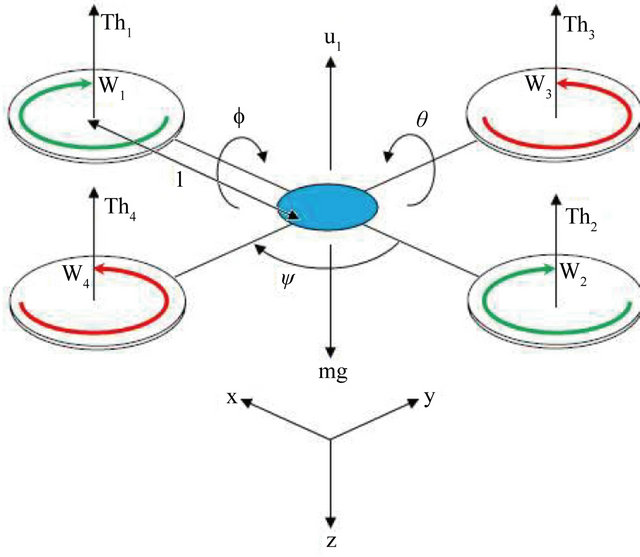
\includegraphics[width=0.70\textwidth]{img/quad_force_diagram.jpg}
\caption{Quadcopter force diagram. Motors and propellors alternate in direction of rotation so that the drone is stable around the vertical axis. The torque generated by each propellor is cancelled by the propellor opposite it \cite{multicopter_dynamics_3}.}
\label{fig:quad_diagram}
\end{figure}\par
\begin{figure}[ht]
\centering
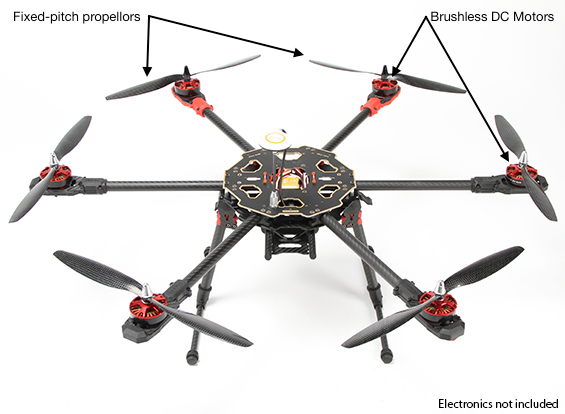
\includegraphics[width=0.70\textwidth]{img/hexacopter.jpg}
\caption{A multicopter with 6 rotors. The brushless DC motors allow for very high speeds and a high degree of control.}
\label{fig:multicopter_hex}
\end{figure}\par
Multicopters use fixed-pitch propellors to correlate rotor speed with force produced. Lift can be controlled by uniformly increasing or decreasing rotor speed across all rotors. To effect a roll or pitch, one side's rotors are spun up and the other side's are spun down so that the net lift remains the same but the craft tilts to the side with less thrust. Multicopters also have the unique ability to yaw in place by spinning alternating rotors faster and slower. Since the rotors alternate in direction of rotation, spinning one set faster creates an imbalance of torque, which makes the whole platform rotate in place \cite{multicopter_dynamics_2}.\par
Multicopters are thus highly maneuverable, but at the cost of flight time and payload capacity. The primary concern when using a multicopter is the flight time. Most commercial multirotors quote flight times in the 10-20 minute range with the best performing drones topping out around 30 minutes \cite{multicopter_comparison}. This is because the power required to spin the electric motors fast enough to get lift can be immense, drawing up to 60 amps on takeoff \cite{multicopter_long_range_mqp}. Ascending from a stationary position draws much more energy than hovering or lateral flying, so multiple takeoffs and landings in one flight will hamper the battery even more. The high current draw of the electric motors necessitates the use of Lithium Polymer (LiPo) batteries that can discharge large amounts of power very quickly. LiPo batteries have another benefit for use in multicopters and that is their low weight.\par
Weight is a very important factor in the operation of a multicopter because the amount of weight to be lifted directly corresponds to the speed the motors must be driven at to achieve lift. Multicopters in general have low payload capacities because any extra weight equates to more power that must be provided by the rotors. In effect, the more weight the drone is carrying, the less flight time it will have. This correlation forces a choice to be made over whether to prioritize flight time or amount of payload supported.\par
The most advantageous aspect of multicopters is their maneuverability. The nature of their control means it is possible to stop and start, hover in place, rotate in place, and quickly change directions and altitudes. In particular, the ability to stop at a point and rotate at a fixed rate is especially unique. To rotate in place, the multicopter increases the speed of all rotors spinning one direction and decreases speed of the other rotors such that the overall lift stays constant, but the torque changes, forcing the whole platform to yaw \cite{multicopter_dynamics}. Deployment of a multicopter is very fast as well: there is nothing that needs assembly prior to flight, and there is no need to find a long open space to takeoff. All that is required procedurally  is powering on the device and setting it on the ground, as multicopters are capable of vertical takeoff and landing (VTOL). The high maneuverability and ease of deployment make for an easy user experience, since control of a drone (with good software) is simple and very responsive. All things considered, the multicopter is a platform that has very good maneuverability, but must sacrifice payload capacity and flight time.
\begin{table}[ht]
\centering
\caption{Multicopter Pros and Cons}
\label{table:multi_pc}
\begin{tabular}{l|l}
  Pros & Cons \\ \hline
  maneuverability & flight time \\
  deployment time & cost \\
   & payload capacity \\
\end{tabular}
\end{table}\par

\section{Chapter Summary}
In this chapter, background information was provided on a range of topics relevant to the undertaken project. The wireless spectrum, divided up into chunks by use, will be the medium for the analysis carried out in this project. Spectrum sensing and localization will be key to achieving the goals of the project. Software Defined Radios are useful for their flexibility around sample processing. Finally, of the flight platforms discussed, multicopters are the only ones with high maneuverability, although they sacrifice flight time and payload capacity to achieve it. This information will allow the informed discussion of implementation of the system for this project.
